\documentclass[svgnames]{beamer}

% https://courses.engr.illinois.edu/cs598jhm/sp2010/Slides/Lecture06.pdf
% https://personal.utdallas.edu/~nrr150130/cs6347/2015sp/lects/Lecture_17_LDA.pdf
% https://www.cs.cmu.edu/~mgormley/courses/10701-f16/slides/lecture20-topic-models.pdf
% 9 http://www.machinelearning.ru/wiki/images/d/d5/Voron17survey-artm.pdf
%http://www.machinelearning.ru/wiki/index.php?title=%D0%92%D0%B5%D1%80%D0%BE%D1%8F%D1%82%D0%BD%D0%BE%D1%81%D1%82%D0%BD%D1%8B%D0%B9_%D0%BB%D0%B0%D1%82%D0%B5%D0%BD%D1%82%D0%BD%D1%8B%D0%B9_%D1%81%D0%B5%D0%BC%D0%B0%D0%BD%D1%82%D0%B8%D1%87%D0%B5%D1%81%D0%BA%D0%B8%D0%B9_%D0%B0%D0%BD%D0%B0%D0%BB%D0%B8%D0%B7
% http://www.machinelearning.ru/wiki/index.php?title=%D0%A2%D0%B5%D0%BC%D0%B0%D1%82%D0%B8%D1%87%D0%B5%D1%81%D0%BA%D0%BE%D0%B5_%D0%BC%D0%BE%D0%B4%D0%B5%D0%BB%D0%B8%D1%80%D0%BE%D0%B2%D0%B0%D0%BD%D0%B8%D0%B5#.D0.92.D0.B5.D1.80.D0.BE.D1.8F.D1.82.D0.BD.D0.BE.D1.81.D1.82.D0.BD.D1.8B.D0.B5_.D1.82.D0.B5.D0.BC.D0.B0.D1.82.D0.B8.D1.87.D0.B5.D1.81.D0.BA.D0.B8.D0.B5_.D0.BC.D0.BE.D0.B4.D0.B5.D0.BB.D0.B8
% https://ppasupat.github.io/a9online/wtf-is/lsa-plsa-lda.html


%assumptions, постановка задачи
%генеративная - хотим найти топики
%pLSA
%недостатки
%LDA
%применения и всякие штуки как это делать по шагам

\usepackage[utf8]{inputenc}
\usepackage[english,russian]{babel}
\usepackage{cmap}
\hypersetup{unicode=true}
\graphicspath{{images/}{slides/images}}

\title[CMTA 06]
{Distributional Semantics}
\subtitle
{Computational Methods for Text Analysis}
\author
{Alena Pestova}
\institute
{HSE Saint-Petersburg}
\date
{08.11.2022}

\subject{natural language processing, text mining}


\newcommand{\tb}[1]{\colorbox{yellow}{#1}\space}
\newcommand{\Sp}[1]{\colorbox{green}{#1}\space}
\newcommand{\Sn}[1]{\colorbox{red}{#1}\space}


\begin{document}

    \begin{frame}
        \titlepage
    \end{frame}


    \begin{frame}{Topic modeling: motivation}
        Suppose you’re given a massive corpora and asked to carry out the
        following tasks:
        \begin{itemize}
            \item Organize the documents into thematic categories
            \item Describe the evolution of those categories over time
            \item Enable a domain expert to analyze and understand the content
            \item Find relationships between the categories
            \item Understand how authorship influences the content
        \end{itemize}

        Topic Modeling:
        A method of    (usually unsupervised)    discovery of latent or hidden structure
        in a corpus
        \begin{itemize}
            \item Applied primarily to text corpora,    but techniques are more general
            \item Provides a modeling toolbox
            \item Has prompted the exploration of a variety of new inference methods to
            accommodate large-scale datasets
        \end{itemize}
    \end{frame}

    \begin{frame}{From words to topics: Multinomial distribution over words}

        \begin{block}{Original Text}
            Карл у Клары украл кораллы, Клара у Карла украла кларнет.
        \end{block}

        \begin{block}{Словарь (распределение)}
            \begin{tabular}[c]{cccccc}
                Карл & у   & Клара & украсть & коралл & кларнет \\
                Карл & у   & Клара & украсть &        &         \\
                2    & 2   & 2     & 2       & 1      & 1       \\
                0.2  & 0.2 & 0.2   & 0.2     & 0.1    & 0.1     \\
            \end{tabular}
        \end{block}
    \end{frame}

    \begin{frame}{Corpus as a mixture of topics (distributions)}
        \footnotesize
        \begin{block}{Topics — events}
            \begin{tabular}[c]{lccccccr}
                Topic          &      &     &       &         &           &           & всего        \\
                \hline
                & Карл & у   & Клара & украсть & коралл    & кларнет   &              \\
                \textit{Карл}  & 0,1  & 0,1 & 0,1   & 0,1     & 0,1       & \alert{0} & \textbf{0,5} \\
                \textit{Клара} & 0,1  & 0,1 & 0,1   & 0,1     & \alert{0} & 0,1       & \textbf{0,5} \\
            \end{tabular}
        \end{block}

        \begin{block}{Topics — common and differences}
            \begin{tabular}[c]{lccccccr}
                Тема            &      &     &       &         &        &         & всего        \\
                \hline
                & Карл & у   & Клара & украсть & коралл & кларнет &              \\
                \textit{Общее}  & 0,2  & 0,2 & 0,2   & 0,2     & 0      & 0       & \textbf{0,8} \\
                \textit{Разное} & 0    & 0   & 0     & 0       & 0,1    & 0,1     & \textbf{0,2} \\
            \end{tabular}
        \end{block}
    \end{frame}

    \begin{frame}{Probabilistic topic models}
        We will look at
        \begin{itemize}
            \item pLSA (Probabilistic Latent semantic analysis)
            \item LDA (Latent Dirichlet Analysis)
        \end{itemize}
    \end{frame}

    \begin{frame}{Some abbreviations}
        \begin{itemize}
            \item D - set of the documents $d$(collection of docs, the corpus)
            \item W - set of all words $w$(vocabulary)
            \item T - set of topics $t$(some latent variable, we do not know)
        \end{itemize}
        Topic:
        \begin{itemize}
            \item \alert{latent} variable (describes words distribution in a corpus)
            \item represents multinomial distribution over words
        \end{itemize}
        we want to find probabilites: $p(w|t)$ and $p(t|d)$

        \begin{itemize}
            \item   toy example of topic family as a distribution over words (p(w|topic=family)):
            [p(dad)=0.3, p(mom)=0.35, p(son)=0.1, p(daughter)=0.1, p(home)=0.25, p(all other words)=0]
            \item example of a document as a distribution over topics (p(t|doc1)):
            [p(family topic)=0.5, p(work topic)=0.3, p(hobby topic)=0.2, p(all other topics)=0]
        \end{itemize}

    \end{frame}

    \begin{frame}{Generative process}
        if we know distributions $p(w|t)$ and $p(t|d)$, then we can generate a document:
        \begin{itemize}
            \item sample a topic for a document from $p(t|d)$
            \item sample words from $p(w|t)$
        \end{itemize}
    \end{frame}

    \begin{frame}
        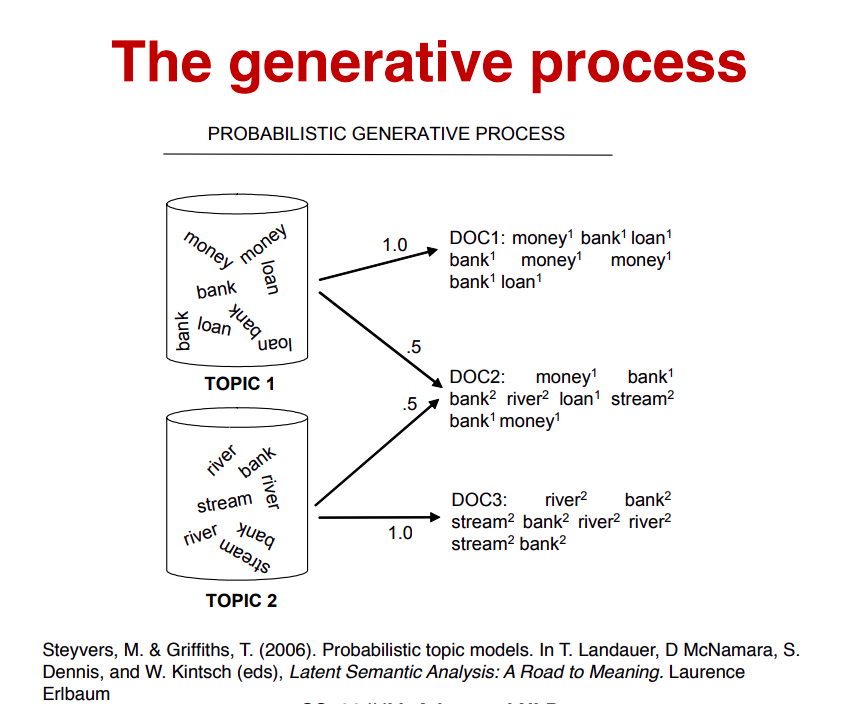
\includegraphics[width=\textwidth]{generative-process}
    \end{frame}

    \begin{frame}
        But we do not know $p(w|t)$ and $p(t|d)$, and we can only see $W$ and $D$ in our data
        (we have some corpus that consists of some number of documents).

        And our task is to find this distributions $p(w|t)$ and $p(t|d)$.

        If we find them, then
        \begin{itemize}
            \item $p(w|t)$ will help us to understand the topics, their interpretation
            \item $p(t|d)$ will help us to understand the documents - what topics are presented in some doc, in what proportions.
        \end{itemize}
    \end{frame}

    \begin{frame}
        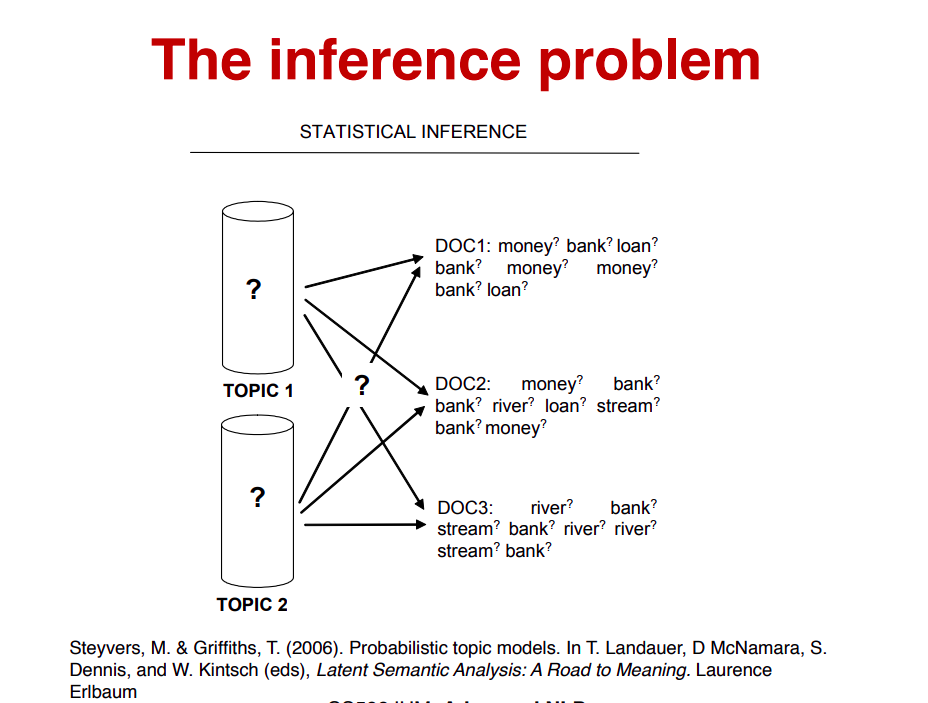
\includegraphics[width=\textwidth]{inference_prob}
    \end{frame}


    \begin{frame}{Basic probabilistic topic models}
        Basic probabilistic topic models are based in the following assumptions:
        \begin{itemize}
            \item the order of documents in the collection is not important
            \item the order of words in the document is not important, document is — «bag of words»;
            \item words found in most documents are not important for defining topics, they are usually excluded from the dictionary and called stop words;
            \item a word in different forms is one and the same word;
        \end{itemize}
    \end{frame}

    \begin{frame}{Basic probabilistic topic models}
        Basic probabilistic topic models are based in the following assumptions:
        \begin{itemize}
            \item a collection of documents can be viewed as a simple selection of document-word pairs $(d,w),\; d\in D,\; w\in W_d.$
            \item each topic $t\in T$ is described by an unknown distribution $p(w|t)$ on the set of words $w\in W$;
            \item each document $d\in D$ is described by an unknown distribution $p(t|d)$ on the set of topics $t\in T$;
            \item conditional independence hypothesis: $p(w|t,d)=p(w|t)$.
            \item To build a topic model means to find the matrices $\Phi = ||p(w|t)||$ and $\Theta = ||p(t|d)||$ from collection $D$.
        \end{itemize}
    \end{frame}


    \begin{frame}
        \frametitle{Probabilistic Latent semantic analysis (pLSA)}
        Hoffman 1999

        Topic:
        \begin{itemize}
            \item \alert{latent} variable (describes words distribution in a corpus)
            \item represents multinomial distribution over words
        \end{itemize}

    \end{frame}

    \begin{frame}
        \frametitle{Generative model pLSA}
        For each \structure{word} in each document:
        \begin{enumerate}
            \item Select <randomly> topic $z$ based on
            the probability distribution of the topics in the collection.
            \item Select <randomly> a word based on distribution
            probabilities of words in topic $z$.
        \end{enumerate}
        Properties:
        \begin{itemize}
            \item one word may belong to several topics (we have distribution $p(w|t) \; t\in T$)
            \item there can be several topics in one document;
            \item the collection has one common topic probability distribution. (!!!)
        \end{itemize}
    \end{frame}

    \begin{frame}
        \frametitle{Graphical model pLSA}
        \centering
        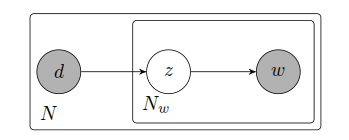
\includegraphics[width=\textwidth]{plsa-model}
    \end{frame}

    \begin{frame}{pLSA: how it is trained}
        we observe $p(w|d)$ (as we see documents that consists of words)
        the model can be trained to maximize the likelihood (maximum likelihood estimation) of:

        $$p(w|d) = \Sigma_{t\in T} p(w|d, t)p(t|d) = \Sigma_{t\in T} p(w|t)p(t|d)$$
        (our probabilistic model)

        $$p(w|d, t) = p(w|t)$$ (conditional independence assumption)

    \end{frame}

    \begin{frame}{pLSA: disadvantages}
        \begin{itemize}
            \item Slow convergency on the big collections of documents
            \item The PLSA algorithm is characterized by overfitting, as well as non-uniqueness and instability of solutions.
            \item The algorithm does not highlight non-topic words.
            In real text, there are terms that do not explicitly refer to any of the topics.
            Accounting for such terms is possible with the help of robust thematic models, in which noise and background components are added.
            \item It cannot assign probabilities to new documents.
        \end{itemize}
    \end{frame}

    \begin{frame}{Latent Dirichlet Allocation (LDA)}
        Assumptions:
        \begin{itemize}
            \item There are $K$ topics in the collection.
            \item Each document is represented as a \structure{mixture of topics}.
            \item «Topic» — multinomial distribution over words. Each word in the vocabulary
            has some weight (probability) \structure{in each topic}.)
        \end{itemize}

        Properties:
        \begin{itemize}
            \item one word may belong to several topics (we have distribution $p(w|t) \; t\in T$)
            \item there can be several topics in one document;
            \item Each document has its own topic distribution (!!!), in one document only some of the topics are represented
        \end{itemize}
    \end{frame}

    \begin{frame}{How LDA differ from pLSA in simple words}
        \begin{itemize}
            \item pLSA - one topic distribution for the whole collection, LDA - each document has its own topic distribution
            \item other differences more related to training (regularization, optimization method (Gibbs sampling), etc.)
        \end{itemize}
    \end{frame}

    \begin{frame}{Generative process of LDA}
        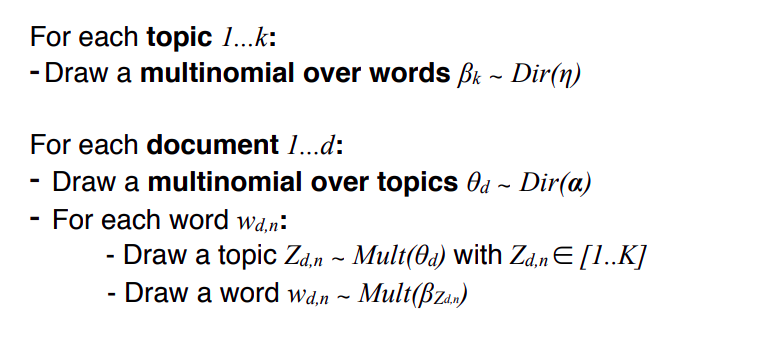
\includegraphics[width=\textwidth]{words-gener-lda}
    \end{frame}

    \begin{frame}{Graphical model of LDA}
        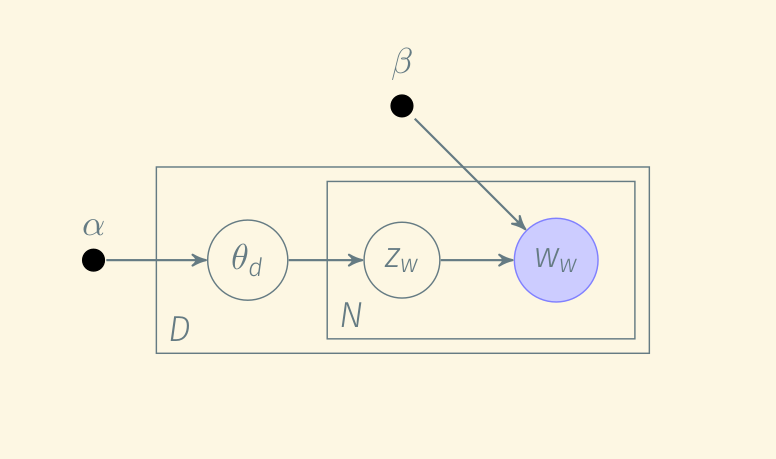
\includegraphics[width=\textwidth]{lda-graph}
    \end{frame}

    \begin{frame}[plain]
        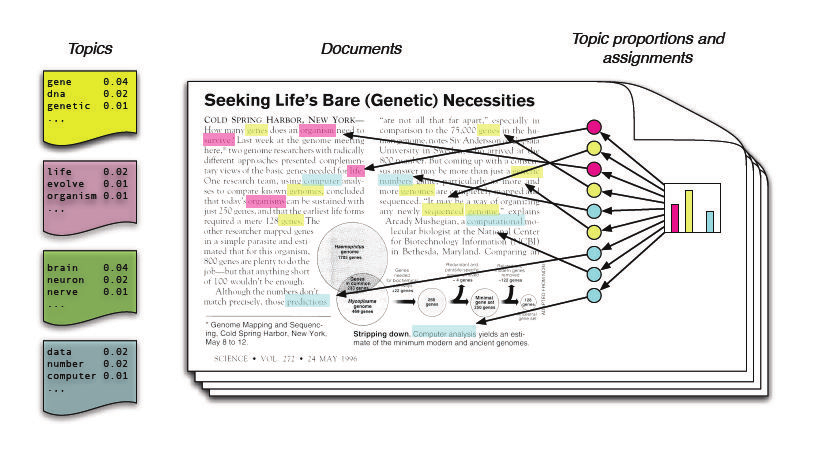
\includegraphics[width=\textwidth]{blei-slide}
        \footnotesize

        Slide by David Blei
    \end{frame}

    \begin{frame}{Pros and cons of LDA}
        Pros:
        \begin{itemize}
            \item It provides better performances than LSA and pLSA.
            \item Unlike pLSA, LDA can assign a probability to a new document thanks to the document-topic Dirichlet distribution.
            \item As a probabilistic module, LDA can be embedded in more complex models or extended. There are extensions that address limitations from previous works.
        \end{itemize}
        Cons:
        \begin{itemize}
            \item The number of topics must be known beforehand.
            \item The bag-of-words approach disregards the semantic representation of words in a corpus, similarly to LSA and pLSA.
            \item It requires an extensive pre-processing phase to obtain a significant representation from the textual input data.
            \item Studies report LDA may yield too general or irrelevant topics.
            \item Results may also be inconsistent across different executions.
        \end{itemize}
    \end{frame}

    \begin{frame}{LDA: hyperparameters}
        \begin{itemize}
            \item $K$ - the number of topics
            \item $alpha$ and $beta$ - parameters of Dirichlet distribution
        \end{itemize}
    \end{frame}

    \begin{frame}{LDA: hyperparameters}
        \begin{itemize}
            \item \url{https://datascienceplus.com/topic-modeling-and-latent-dirichlet-allocation-lda/}
        \end{itemize}
    \end{frame}

    \begin{frame}{Topic modeling: texts preparation}
        \begin{enumerate}
            \item Preprocessing
            \item Segmentation
        \end{enumerate}
    \end{frame}

    \begin{frame}{Preprocessing: stop-words}
        \begin{itemize}
            \item Static list:
            \item Dynamic list:

            \begin{itemize}
                \item Too frequent words (N most frequent)
                \item Too rare words (threshold: appear less than in N docs)
                \item Too short (less then N letters)
            \end{itemize}
        \end{itemize}
    \end{frame}

    \begin{frame}{More preprocessing}
        In TM, it can be a good idea to delete even more words. For example:
        \begin{itemize}
            \item Not nouns (ot not nouns and adjectives)
            \item Proper nouns (names)
        \end{itemize}
    \end{frame}

    \begin{frame}{Segmentation}
        Size of the document is important.
        \begin{itemize}
            \item Divide long texts (for ex, novels)
            \item Merge short texts (for ex, text messages)
            \item Optimal(?) text length — 100—1000 words (from abstract to article)
        \end{itemize}
        \centering
        \alert{The main principle is the unity of context.}
    \end{frame}


%\begin{frame}{Again about TM}
%  \begin{itemize}
%    \item in real
%    \item Мы не можем наблюдать «темы».
%    \item Мы наблюдаем только документы.
%    \item LDA должен «восстановить» \structure{дискурсы}, которые
%      породили документы.
%    \item Невозможно точно восстановить темы: слишком много неизвестных.
%  \end{itemize}
%\end{frame}

    \begin{frame}{Output of LDA}
        You will see some lists like this:
        \includegraphics[width=\textwidth]{topic-r}

        (most probable words for each topic)
        So, you will probably try to interpret all this topics, drop the noisy ones and then try to do smth else.


        You also can obtain: the probability of each topic in the document. So, you can:
        \begin{itemize}
            \item calculate the topics proportions in the documents/in some groups/in different time periods
            \item look at the co-occurence of the topics in the documents
            \item etc.
        \end{itemize}
    \end{frame}

%    \begin{frame}{Интерпретация}
%        \footnotesize
%        \begin{block}{Фрида Вигдорова, Это мой дом (1961)}
%            Меня вызвали в <>. Я шел по длинному \textcolor{orange}{полутемному коридору}, и вдруг
%            откуда-то \textcolor{orange}{выскочила} девчонка лет одиннадцати.
%
%            <...>
%
%            Вызвала меня <>. Когда я \textcolor{orange}{вошел}, она бегло
%            посмотрела в мою сторону, уронила: <...> – Привычку командовать надо
%            оставить, то-ва-рищ <>! Я вижу, что слухи о вашем самомнении не
%            преувеличены. Я вызвала вас для того, чтобы сказать: неприлично
%            \textcolor{cyan}{директору} детдома заниматься саморекламой!
%
%            И вот тут я делаю непозволительную глупость. При этом имени я встаю и,
%            не прощаясь, покидаю кабинет <>. <...>
%            Иду по \textcolor{orange}{коридору}, стиснув зубы, и злюсь на себя.
%
%            Оборачиваюсь. Девчонка со всех ног \textcolor{orange}{удирает} от меня и, еще два раза
%            выкрикнув ехидным голосом: «Цыган! Цыган!» – \textcolor{orange}{скрывается за дверью} в
%            конце \textcolor{orange}{коридора}.
%
%            – Ну нет! Не уйдешь!
%
%            Иду за ней, дергаю \textcolor{orange}{дверь} – она \textcolor{orange}{заперта} изнутри. Стою тихо, жду. \textcolor{orange}{Дверь
%            чуть приоткрывается}, \textcolor{orange}{в щелку} виден кончик вздернутого носа, и \textcolor{orange}{дверь
%            снова захлопывается}.
%        \end{block}
%    \end{frame}


    \begin{frame}{Interpretation}
        \only<2->{
            \begin{columns}
            \column{.25\textwidth}
            
\includegraphics[width=\textwidth]{snape}
            \column{.75\textwidth}
            {\centering\LARGE\alert{Interpretation:\\ \only<3>{portrait descriptions}}\par}
    \end{columns}
}

\bigskip

\textcolor<2>{orange}{eye} \textcolor<3>{cyan}{face lip hand} \textcolor<2>{orange}{glance} \textcolor<3>{cyan}{eyebrow hair voice smile nose forehead}
\textcolor<2>{orange}{взглядывать} \textcolor<3>{cyan}{щека} \textcolor<2>{orange}{подымать} темный \textcolor<3>{cyan}{плечо} \textcolor<2>{orange}{строгий} широкий \textcolor<3>{cyan}{рот}
повертываться черный \textcolor<3>{cyan}{ухо палец} открытый словно \textcolor<2>{orange}{выражение} высокий
бледный густой весить прямой \textcolor<3>{cyan}{подбородок} звать угол чувствовать
круглый вспыхивать похожий покраснеть сводить слегка несколько
спокойно дело \textcolor<3>{cyan}{eyelash} левый живой поглядеть успевать
\end{frame}


\begin{frame}{Model evaluation}
\begin{itemize}
\item Human judgment of
\begin{itemize}
\item Topics interpretability
\item sufficient generality / specificity of topics (based on the task)
\end{itemize}
\item Measures of topics coherence (perplexity/coherence)
\item * Assessment using metrics of the final task, if such a task exists
\end{itemize}

\end{frame}

\begin{frame}{Model evaluation: Varieties of bad topics}
\footnotetext{\fullcite{mimno2011optimizing}}
\begin{description}
\item[Chained] every word is connected to every other word through
some pairwise word chain, but not all word pairs make sense.
\alert{fatty $\leftarrow$ acids $\rightarrow$ nucleic}
\item[Intruded] either two or more unrelated sets of related words,
joined arbitrarily, or an otherwise good topic with a few
“intruder” words.
\item[Random] no clear, sensical connections between more than a few
pairs of words
\item[Unbalanced] the top words are all logically connected to each
other, but the topic combines very general and specific terms
\end{description}
\end{frame}


%\begin{frame}
%  \frametitle{Topic size}
%  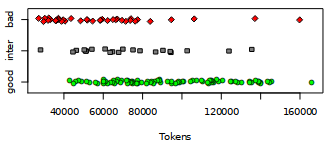
\includegraphics[width=\textwidth]{topicsize}
%\end{frame}


\begin{frame}{Model evaluation: Topic coherence}

Topic Coherence measures score a single topic by measuring the degree of semantic similarity between high scoring words in the topic.
These measurements help distinguish between topics that are semantically interpretable topics and topics that are artifacts of statistical inference.
$$
C(t; V^{(t)}) =\sum_{m=2}^{M} \sum_{l=1}^{m-1} \log\frac{D(w_{m}^{(t)},w_{l}^{(t)})+1}{D(w_{l}^{(t)})}
$$, где
\begin{itemize}
\item $D(w)$ — document frequency of the word $w$
\item $D(w,w')$ — joint document frequency of the words $w$ и $w'$
\item $V^{(t)}=(v_1^{(t)},\dots, v_M^{(t)})$ — list of top-M most probable words in the topic t
\end{itemize}
\end{frame}
%
%\begin{frame}{Topic coherence}
%  \frametitle
%  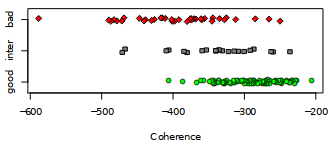
\includegraphics[width=\textwidth]{coherence}
%\end{frame}

\begin{frame}{What is K (the number of topics)?}
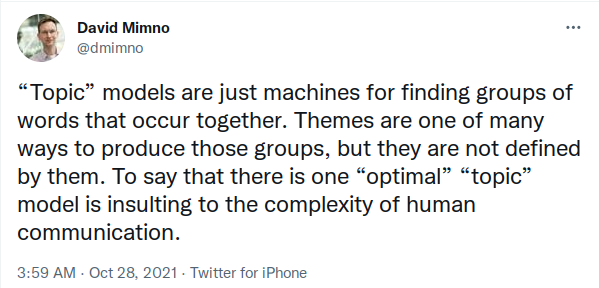
\includegraphics[width=\textwidth]{dmimno-on-tm}
\end{frame}

\begin{frame}{LDA: summary}
    \begin{itemize}
        \item Distributional Hypothesis
        \item Corpus
        \item Defining the documents
        \item Selection and normalization of words
        \item training LDA model, tuning hyperparameters)
        \begin{itemize}
            \item Document-term matrix
            \item Topic as a multinomial distribution over words
            \item Distribution of topics in the documents with Dirichlet
        \end{itemize}
        \item Interpretation
    \end{itemize}
\end{frame}

\begin{frame}
Some links with simple (or not) explanations:
\begin{itemize}
\item about lda and other algorithms: \url{https://towardsdatascience.com/topic-modeling-with-lsa-plsa-lda-nmf-bertopic-top2vec-a-comparison-5e6ce4b1e4a5}
\item nice explanation of $\alpha$ and $\beta$ parameters in LDA model in the beginning of the algorithm: \url{https://datascienceplus.com/topic-modeling-and-latent-dirichlet-allocation-lda/}
\item topic coherence with examples of tuning hyperparameters (though in Python) : \url{https://towardsdatascience.com/evaluate-topic-model-in-python-latent-dirichlet-allocation-lda-7d57484bb5d0}
but there are explanations of topic coherence. BUT such tuning hyperparameters with topic coherence measures may be not as good idea -
it does not guarantee that interpretability of topics will increase.
\item about TM in simple words in russian: \url{https://sysblok.ru/knowhow/kak-ponjat-o-chem-tekst-ne-chitaja-ego/}
\end{itemize}
\end{frame}

\end{document}
